\documentclass[a4paper,12pt]{article}
\usepackage{amssymb,amsmath}
\usepackage[utf8]{inputenc}

% Setup for fullpage use
\usepackage{fullpage}
\usepackage{graphicx}
\usepackage[ruled,vlined,english]{algorithm2e}
\usepackage{listings}
\usepackage{xcolor}

\usepackage[english]{babel}

\title{
{\Huge Scheduling project}\\
\smallskip
}

\author{
Group member:\\
Vincent Gailly\\
Maxime Renversez
\smallskip
}


\date{ Academic year 2021-2022\\
Master in computer sciences \\
\vspace{1cm}
Faculty of sciences, ULB}

\usepackage{amstext} % for \text macro
\usepackage{array}   % for \newcolumntype macro
\newcolumntype{L}{>{$}l<{$}} % math-mode version of "l" column type

\begin{document}
\maketitle
\newpage
\tableofcontents
\newpage

\section{Introduction}

This project is divided into three parts. We have to implement an FTP scheduler, a graphical tool to visualize the result of the scheduling and the Audsley algorithm. In this report, we will explain how we did that. In order to do that, we are going to discuss about the structure of our project, the implementation of the FTP scheduler and Audsley algorithm. We will also provide you an user guide. Before concluding, we will explain the difficulties that we met during the project.      

\newpage

\section{Project structure}

We have decided to do the project in object oriented programming with Python. We have created different classes wich each represent an object and a file which runs the project. We have created these objects : \\
\begin{itemize}
\item[-] a job 
\item[-] a task 
\item[-] a scheduler 
\item[-] a object  to visualize the scheduling 
\item[-] ...
\end{itemize}

\smallskip
\noindent
A job is caracterized by a release date, a computationnal time and a deadline. 

\smallskip 
A completer quand audsely sera fini  + faire diagramme uml !! 

\newpage

\section{User guide}

\newpage

\section{FTP scheduler}
\subsection{Algorithm}

\begin{lstlisting}
1 def startScheduler(self):
2	time = 0
3	job_duration = 0
4	job_start = 0 
5	task_number = 1
6	feas_int = self.computeFeasibilityInterval()
7	while time <= feas_int and self.verifyDeadlines(time):
8		task_to_execute = self.canBegin(time)
9		if task_to_execute != -1:
10			if task_to_execute != task_number:
11				if task_number != -1:
12					self.tasks_list[task_number - 1].schedule_solution.append((job_start,job_duration))
13					job_duration = 1
14					job_start = time
15				else:
16					job_start = time
17					job_duration = 1
18			elif task_number == task_to_execute:
19				job_duration += 1
20			self.executeTask(task_to_execute)
21		else:
22			self.tasks_list[task_number - 1].schedule_solution.append((job_start,job_duration))
23			job_duration = 0
24			job_start = 0 
25		task_number = task_to_execute
26		time += 1
27	return not time < feas_int
\end{lstlisting}

\smallskip
\noindent
The purpose of this algorithm is to execute the FTP scheduler and returns ``TRUE'' if it ends correctly and ``FALSE'' otherwise. If it returns ``FALSE'' it means that the set of tasks are not schedulable. The variable \textbf{time} represents the current time in the scheduler. The variables \textbf{job\_duration} and \textbf{job\_start} represent the duration of the execution of one job and at which time the job is executed for the first time (these variables allow us to keep a track of the execution of all the jobs of all the tasks). The variable \textbf{task\_number} is the number of the task which has its job that is being executed. The variable \textbf{feas\_int} represents the upper bound of the feasibility interval which is calculated by the method ``computeFeasibilityInterval()''. The while loop will be explained in subsection 4.2. (Parler du task\_number $=$ 1 et pq ca ne gene pas)
\newpage
\subsection{Explanations of the while loop}

To stay in the loop, two conditions must be respected : \\
\begin{itemize}
\item[-] The time must be less or equal to the upper bound of the feasibility interval.
\item[-] No deadlines are missed. 
\end{itemize}

\smallskip
\noindent
When the program enters in the loop, it first calculates which task can execute its job and stores its number in the variable \textbf{task\_to\_execute}. It is done by the method ``canBegin(time)'' which takes the current time in parameter and returns a task number. This method respects the task priorities. For example, if two tasks can execute their job at the same moment, it returns the task number which has the higher priority. But if no tasks can execute a job (it is when all the jobs have finsihed their executions and the new jobs are not yet released), it returns ``-1''. Once we know which task can execute its task, we must dinstinguish four cases. Before explaining these cases, just a reminder of the difference between \textbf{task\_number} and \textbf{task\_to\_execute}. We can see the first one as the ``past'' (at time t-1) and the second one as the ``present'' (at time t).

\subsubsection{Case 1}

\begin{figure}[h!]
  \centering
  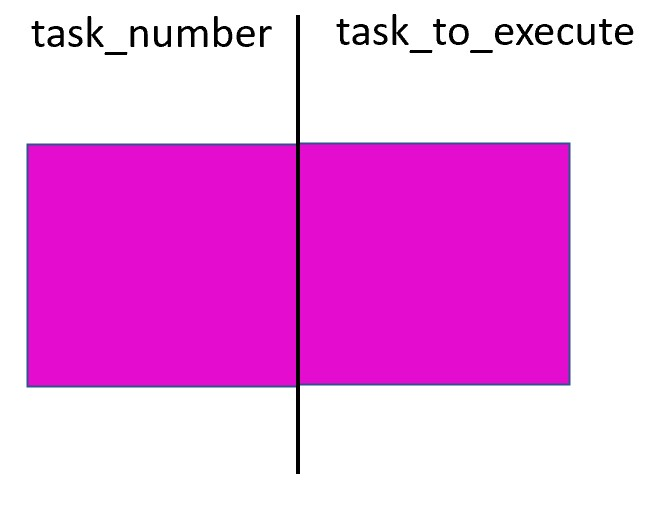
\includegraphics[width=0.5\textwidth]{Pictures/Case1.jpg}
  \caption{Case 1}
  \label{fig: Case 1}
\end{figure}

\smallskip
\noindent
It is the case when the job executed at time t-1 is the same as the job executed a time t (see line 18 - 19 in the algorithm). It is the easiest case. Indeed, we just need to increment the duration of the execution of job because the job will be executed one more unit of time. 


\newpage

\subsubsection{Case 2}

\begin{figure}[h!]
  \centering
  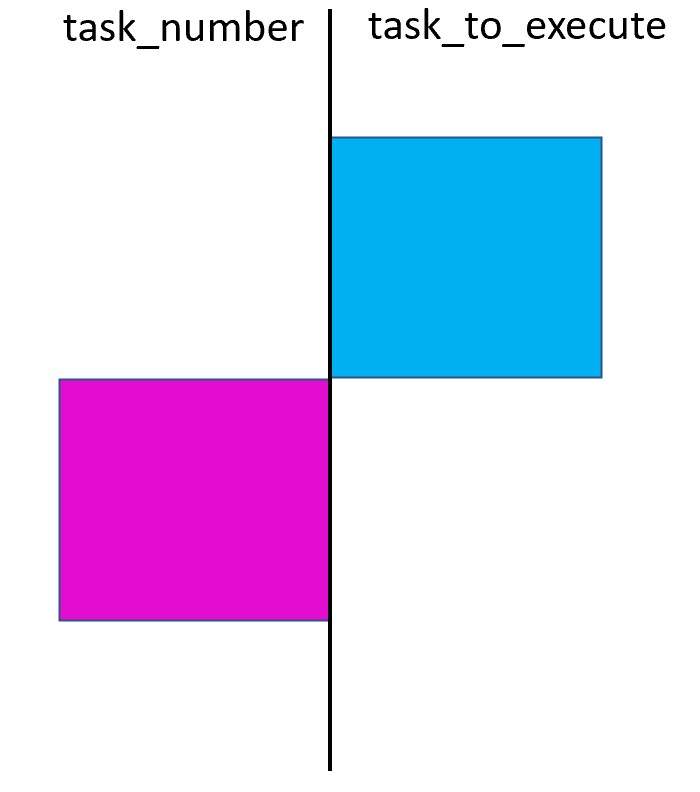
\includegraphics[width=0.5\textwidth]{Pictures/Case2.jpg}
  \caption{Case 2}
  \label{fig: Case 2}
\end{figure}

\smallskip
\noindent
It is the case when at time t-1 the job of a task is executed and at time t the job of another task is executed (see line 12 - 14 in the algorithm). In this case, we add a tuple composed of the start time of the job (given by the variable \textbf{job\_start} and its duration (given by the variable \textbf{job\_duration}) in a list belonging to the task whose the job was executed at time t-1. ET ON REMETS LES VALEURS DES VARIABLES 0 JOUUR


\section{Audsley’s priority assignment}

\newpage

\section{Difficulties}

\newpage

\section{Conclusion}

\end{document}